\section{Data set and imputation}
The dataset consists of phenotype and genotype data of 1,008 prototrophic haploid \emph{Saccharomyces cerevisiae} segregants derived from a cross between a laboratory strain and a wine strain strain. It contains 11,623 unique genotypic markers obtained via short-read sequencing for all 1,008 segregants (no missing genotypes). For phenotyping, segregants were grown on agar plates under 46 different conditions, including different temperatures, pH and nutrient addition (see labels in Figure~\ref{fig:traitcorrelations}). The phenotypes were definded as end-point colony size normalized relative to growth on control medium. For the remainder of this chapter, a trait is defined as the normalised growth size in one conditions. Out of the 1,008 segregants, 303 segregants were phenotyped for all 46 traits.

\subsection{Missing data mechanism} 
In order to gain an understanding of the dataset, I first looked at the frequencies and distribution of missing values. There are 135 different combinations of missing values across the samples and the missing phenotypes are not evenly distributed (Figure~\ref{fig:missingness-all}). Some traits such as cobalt chloride are present for almost all samples while others such as sorbitol or raffinose are lacking in more than a third of the samples. I used Little's global test for MCAR to analyse wether these observed data patterns can be acocunted for through a MCAR mechanism. It tests the null hypothesis that the data is MCAR \citep{Little1988,Beaujean2015}, which can in this case be rejected with a p-value of 2E-34 (based on a \(\chi^2\) dsitribution, \(\chi^2=5,902\), \(df=4,63\)). 

\begin{figure}[p]
	\centering
	\begin{subfigure}[b]{1\textwidth}
		%\hspace{3cm}
		\center
	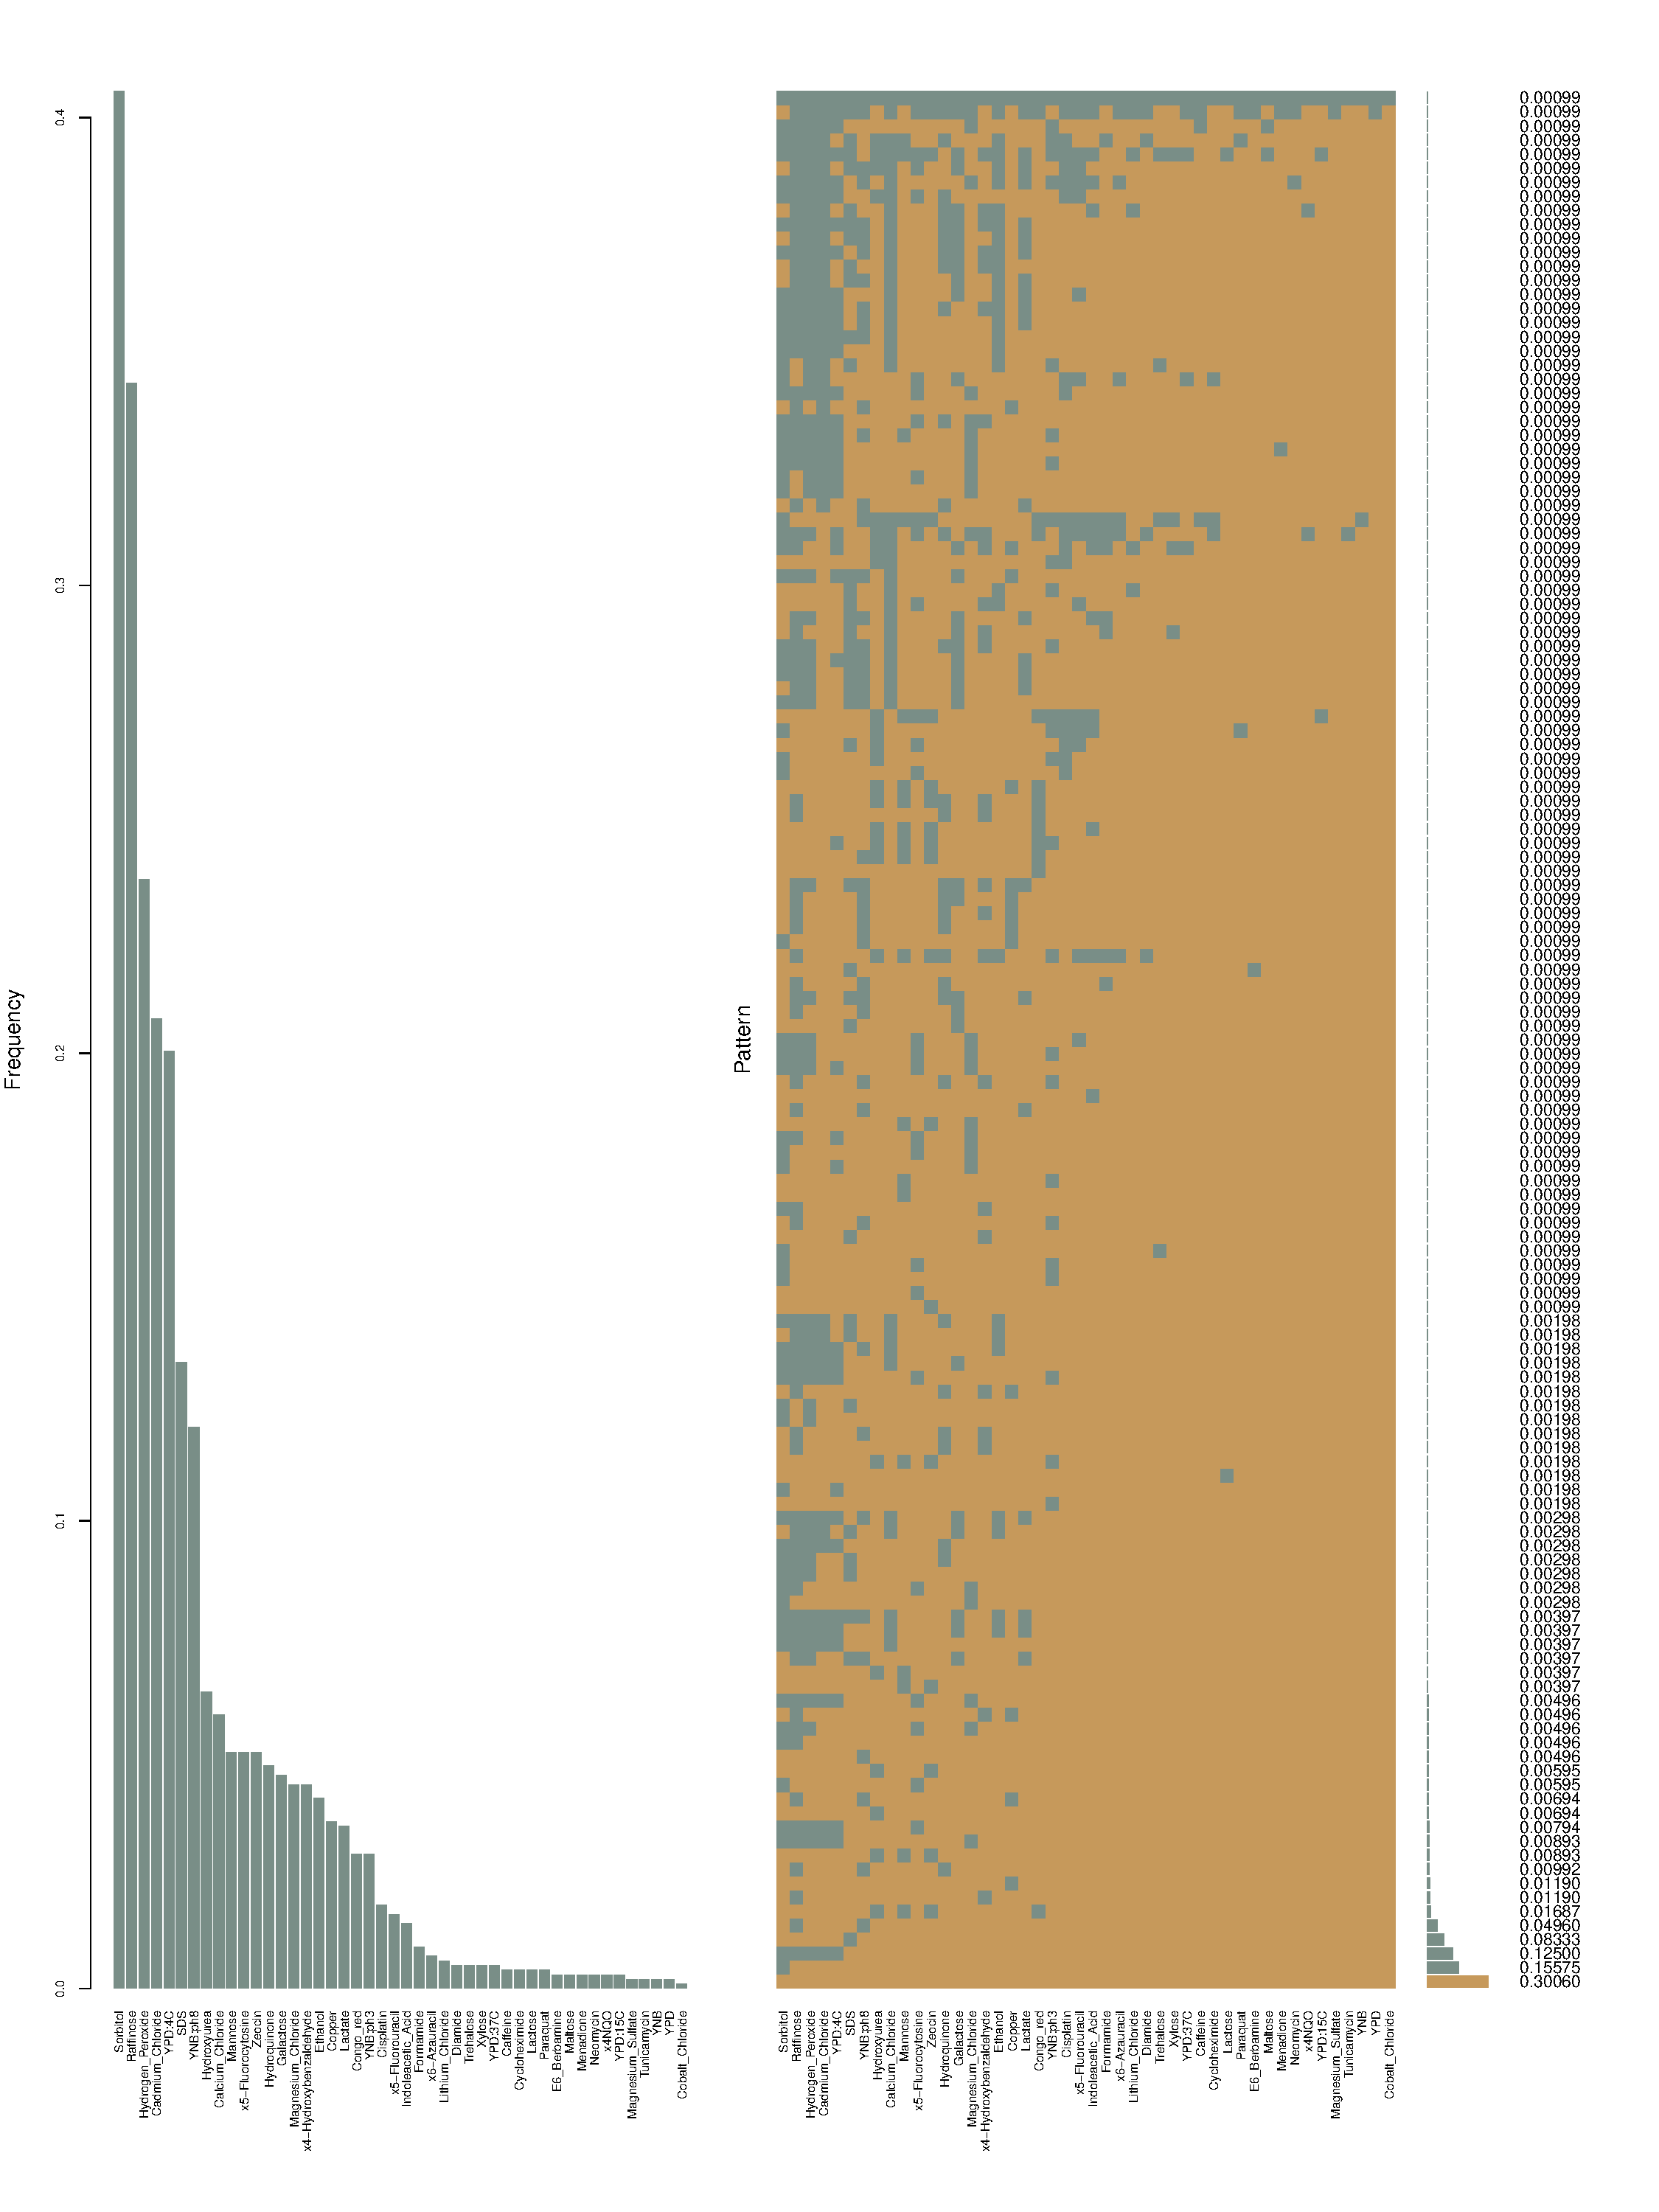
\includegraphics[trim = 0mm 0mm 0mm 0mm, clip, scale=0.8]{Chapter2/Figures/missing_data_pattern.pdf}
	\caption{\textbf{Full dataset}}
 		\label{fig:missingness-all}
	\end{subfigure}
	\\
	\begin{subfigure}[b]{1\textwidth}
		%\hspace{3cm}
		\center
	\includegraphics[trim = 0mm 0mm 0mm 20mm, clip, scale=0.8]{Chapter2/Figures/missing_data_pattern_simulated.pdf}\\
	\caption{\textbf{Simulated  dataset}}
 		\label{fig:missingness-sample}
	\end{subfigure}
	\caption[Frequencies and distributions of missing values in the yeast phenotype data]{\textbf{Frequencies and distributions of missing values in the yeast phenotype data.} In both panels, the aggregation plot (middle) depicts all existing combinations of missing (blue) and non-missing (orange) values in the traits. The bar chart on its right shows the frequencies of occurrence of the different combinations. The histogram on the top shows the frequency of missing values for each trait. (R Package: \emph{VIM} \citep{Templ2012}). (a) The full dataset contains normalised colony sizes for growth in 46 different conditions of 1,008 genotyped yeast segregants. 306 segregants are fully genotyped (bar chart, orange bar). (b) Fully-phenotyped dataset of 306 segreagants with simulated missing values based on the observed missingness pattern for the entire pool of 1,008 segregants.}
 	\label{fig:missingness}
\end{figure}

Determining if data is MAR or MNAR cannot be tested for formally and relies on approximate measures and assumptions based on the experimental procedures \citep{SchaferGraham2002,Garson2015,Templ2012}. Garson suggests to use significance tests of missingness \citeyear{Garson2015}. If it can be demonstrated that one or more variables in the dataset are significantly correlated with missing values, missingness may be predictable, which is the requirement for imputing MAR data. In order to test for predictable missingness, I created an indicator matrix for the phenotype matrix, where observed values where encoded as 0 and missing values as 1. For each of the 46 traits in the dataset I correlated the observed values across all samples with each column of the indicator matrix, i.e. the missingness patterns per trait. If all values were observed for a given trait i.e. all values in the incator matrix in this column were equal to 0, then the correlation between the trait and the missingness was set to NA. Figure~\ref{fig:missingnesscorrelations} shows these correlation patterns between the phenotypes and the missing values per trait. The p-values of the correlations were adjusted for multiple testing via Benjamini and Hochbergs method \citep{Benjamini1995} and only significant correlations are depicted (\(FDR < 0.2\).  For traits like cobalt chloride and magnesium sulfate where little data is missing, many entries are NA. Overall, fo a number of traits and missingness patterns, I found sufficient evidence for predictable missingness and MAR assumptions for further analyses were considered valid. Most importantly, for data with MAR, the missing data mechanism is ignorable for maximum likelihood based methods and no further adjustments for the mechansims have to be made in the modeling \citep{Rubin1976,Little1988}. Thus, the MAR assumption of missingness in the yeast data allows for imputation via the likelihood-based method of multiple imputation.


\begin{figure}[hbtp]
	\centering
	\includegraphics[trim = 0mm 0mm 0mm 0mm, clip, width=0.9\textwidth]{Chapter2/Figures/correlation_missingness.pdf}
	\caption[Correlations of observed phenotypes with missing data values]{\textbf{Correlations of observed phenotypes with missing data values}. For each trait, Spearman's rank correlation coefficient \(\rho\) was computed with each column of the indicator matrix of the phenotypes, containing 0 for observed values and 1 for missing values. The p-values of the correlations were adjusted for multiple testing according to Benjamini and Hochberg's method \citep{Benjamini1995}. The strength and the direction of significant correlations (\(FDR < 0.2\)) are depicted above., with the original phenotypes in rows and the indicator matrix of the phenotypes across columns. Unsignificant correlations are left blank. Grey squares indicate NA, i.e. columns in the indicator matrix for which no traits were missing when correlated with the observed values for a given trait.(R Package: \emph{corrplot}).}
 	\label{fig:missingnesscorrelations}
\end{figure}

\subsection{Imputation via MICE} 
Before imputing the missing values in the dataset, I wanted to understand which missing trait values can be reliable imputed and find the best parameter settings for the imputation. In order to do this, I needed a fully phenotyped dataset with the same structure as the yeast dataset, where missing values could be introduced, imputed and subsequently compared to the true values. I chose a simple approach and used the subset of 303 fully phenotyped samples and introduced missing values with a similar pattern of missingness as observed in the original dataset. The results for the real (Figure~\ref{fig:missingness-all}) and simulated (Figure~\ref{fig:missingness-sample}) dataset are similar in terms of frequencies and combination of missing/non-missing traits .

I used this simulated dataset as input to the imputation framework based on multiple imputation by chain equations (MICE) \citep{vanBuuren2011}. 
\paragraph{MICE.} MICE belongs to the general class of multiple imputation frameworks, where several imputed versions of the dataset are generated. The imputations are done separately for each variable. The imputed values are chosen from plausible values drawn from a distribution that is specific for that variable, in this case for each trait. This distribution is derived from the dataset \(X \in R^{n,p}\) itself,  with \(X = (X_\text{miss}, X_\text{obs})\) (the missing and the observed parts of the data), the binary indicator matrix for missingness \(M \in R^{n,p}\) and a set of predictor variables \(Z\). The MICE algorithm is usually divided into four steps \citep{Rubin1978,vanBuuren1999,Pigott2001,}:
\begin{enumerate}
\item Specify the posterior predictive density \(p(X_\text{miss} | Z, M)\) given the non-response mechanism  \(p(M | X)\)  and the complete data model  \(p X)\).
\item Draw imputations from this density to produce \(m\) complete data sets. 
\item Perform \(m\) complete-data analyses on each completed data matrix. 
\item Pool the \(m\) analyses results into final point and variance estimates.
\end{enumerate}
Garson describes the possibilty of switching step 3 and 4 \citeyear{Garson2015}, where the multiple imputations are first pooled and the subsequent analyses run on the pooled estimates. Employing this approach allows me to  obtain reliable imputation estimates while having to estimate the variance components via LiMMBo only once. As described in the previous chapter, LiMMBo strongly reduces the computation time for the variance decomposition, but it is still the time-consuming factor in the analysis. 

\noindent The two main choices in applying MICE for imputation have to be made in step 1: the form of the imputation model and the choice of predictor variables. 

\paragraph{Imputation model.} From the different imputation models available (examples described in \citep{vanBuuren2011}, I found multivariate data predictive mean matching (PMM) a fast and sensible imputation model. PMM is a semi-parametric method which preserves non-linear relations in the data \citep{Little1988,vanBuuren2011}. In brief, PMM finds the mean and covariance of the multi-variate distribution \(X\) with missing values (often simply based on the complete cases). Subsequently, for each incomplete sample it predicts the missing values \(X_\text{miss}\) based on \(X_\text{obs}\)  and the provided predictor variables \(Z\). In addtion, values of the complete samples for the same set of \(X_\text{miss}\) are predicted. The predicted values of the incomplete sample are than matched to the predicted values of the complete samples and the closest match is chosen. The imputed values for the incomplete sample are set to those of the closest match\citep{Little1988}. 

\paragraph{Predictor variables.} As many predictor variables as possible should be included in the imputation to obtain the least amount of bias and maximal certainty about the predictions \citep{Collins2001}. In addition, Schafer showed that using this strategy makes MAR assumptions more plausible \citep{Schafer1997}. However, not all predictors will be relevant and the choice of predictors can be done on a per-variable level. In order to select suitable predictors for each trait, I first computed the pairwise Spearman correlation coefficient \(\rho\) for all traits across the 303 fully-phenotyped segregants. Some of the traits like cadmium chloride or neomycin show very little correlation to any of the other traits, while many of the traits based on growth on different carbohydrate resources form a large cluster of moderate to strong correlation (Figure~\ref{fig:traitcorrelations}). 
I tested several sets of predictor variables, either using all traits as predictors or chosing predictors based on the pairwise \(\rho\) of the traits. For each trait, I included predictors that showed a correlation higher than a predefined threshold (\(\rho =\left\{0.1, 0.2, 0.3\right\}\). In addition, I restricted the predictors to traits that had been measured in at least 20\% of the samples in the dataset. This excluded cadmium chloride  (0.21\% missing), hydrogen peroxide (0.24\%), raffinose (0.34\%), sorbitol (0.41\%) and YPD:4C (0.20\%) as predictor variables, but did not exclude them from being imputed.

\begin{figure}[hbtp]
	\centering
	\includegraphics[trim = 0mm 0mm 0mm 0mm, clip, width=0.9\textwidth]{Chapter2/Figures/correlation_pheno_noNA.pdf}
	\caption[Pairwise correlations of 46 growth traits in \emph{Saccharomyces cerevisiae}]{\textbf{Pair-wise correlations of 46 growth traits in \emph{Saccharomyces cerevisiae}.} For each trait pair, Spearman's rank correlation coefficient \(\rho\) and the p-values of the correlation were computed. The p-values were adjusted for multiple testing according to Benjamini and Hochberg's method \citep{Benjamini1995}. The strength and the direction of significant correlations (\(p < 0.05\)) are depicted above. Unsignificant correlations are left blank. The traits are clustered based on complete-linkage clustering of \((1-\rho)\) as distance measurement (R Package: \emph{corrplot}).}
 	\label{fig:traitcorrelations}
\end{figure}

Further parameters for MICE are the number of multiple iterations \(m\) (set to \(m=20\)) and the number of iterations \(maxit\) (set to \(maxit=30\)). For each predictor set-up, I initiated MICE with the same seed for the random number generator to ensure comparability. After imputation, I evaluated the goodness of the imputation  by computing the Spearman correlation of the imputed values (averaged across iterations \(m\)) to the experimentally observed ones (Figure~\ref{fig:mice}). Traits where the imputed values correlated to the original ones by more then 95\% in at least one of the predictor set-ups were retained in the analysis. For five traits (cadmium chloride, hydrogen peroxide, raffinose, YNB:ph8, YPD:4C), no suitable predictors could be determined and these were excluded from further analyses (Figure~\ref{fig:mice}, red labels). For each trait, I chose the predictor scheme that yielded the highest correlation between the imputed and observed data for the imputation of missing values in the full dataset. Missing values were imputed in segregants that were phenotyped for at least 80\% of the traits. The final dataset contained 981 segregants with phenotypes for 41 traits each. 
 	
\begin{figure}[hbtp]
	\centering
	\includegraphics[trim = 0mm 0mm 0mm 0mm, clip, width=01\textwidth]{Chapter2/Figures/imputation_correlation_median_imputationvalue.pdf}
	\caption[Correlation between imputed and experimentally observed trait values]{\textbf{Correlation between imputed and experimentally observed trait values.} In the subset of 306 fully phenotyped samples, missing values were introduced and subsequently imputed via MICE. Different predictor sets were tested based on Spearman's rank correlation coefficient: traits were considered predictors if their correlation with the target trait was greater than a given threshold. For each predictor setup (all traits as predictors and predictors passing the corrleation threshold \(\rho =\left\{0.1, 0.2, 0.3\right\}\),   \(m=20\) multiple imputations and \(maxit=30\) iterations of MICE were conducted. The goodness of the imputation was evaluated by computing the correlation of the imputed values (averaged across iterations \(m\)) to the experimentally observed ones. Traits with at least one correlation greater than the 0.95 (black vertical line) were retained in the dataset. For traits labeled in red, the imputation was considered to be unreliable and the traits were excluded from further analyses (R Package: \emph{mice} \citep{vanBuuren2011}).}
 	\label{fig:mice}
\end{figure}


